\documentclass[a4paper,10pt,UTF8]{scrartcl}
\usepackage{xltxtra}
\usepackage[]{xkeyval,polyglossia}
% \setmainlanguage[spelling=new]{german}
\usepackage[b5paper,top=2cm, bottom=2cm, left = 2.5cm, right=2cm]{geometry}
\usepackage[]{csquotes}
\usepackage[]{titlesec}
\usepackage[]{url}
\usepackage[]{paralist}
\usepackage[absolute]{textpos}
\usepackage[]{rotating}
\usepackage[]{scrpage2}
\usepackage[]{blindtext}
\usepackage{ctex}
\usepackage{graphicx}
\usepackage{hyperref} 
% \usepackage{abstract}
% \setlength{\baselineskip}{10pt}
\usepackage{indentfirst}
\usepackage{enumerate}
\usepackage{fontspec}


% \usepackage[a4paper,left=2.8cm,right=2.8cm,top=2.5cm,bottom=2.5cm]{geometry}
\usepackage{graphicx}
\usepackage{pythonhighlight}
\usepackage[mathscr]{eucal}
\usepackage{mathrsfs}
\usepackage{booktabs}
\usepackage{capt-of} 
\usepackage{hyperref} 
\usepackage{abstract}
\usepackage{amsmath}
\usepackage{listings}
\usepackage{color}
\usepackage{caption}
\usepackage{subfigure}
\usepackage{enumerate}
\usepackage{amsfonts} 
\usepackage{float}


\pagestyle{scrheadings}
\setheadsepline[\textwidth]{0.25pt}{}
\ohead{\headmark}
\ofoot[\pagemark]{\pagemark}
\cfoot{}
\chead{}

\ihead{Kodak Strategic Analysis}


\usepackage{xcolor}
\definecolor{msdarkblue}{RGB}{54,95,145}
\definecolor{msblue}{RGB}{79,129,189}
%\titleformat{\section}[form]{layout}{labellayout}{abstand}{davorcode}[danachcode]
\titleformat{\abstract}[hang]{\color{msdarkblue}\Large\sffamily\bfseries}{}{0pt}{\vspace*{-6pt}}
\titleformat{\section}[hang]{\color{msdarkblue}\Large\sffamily\bfseries}{}{0pt}{\vspace*{-6pt}}
\titleformat{\subsection}[hang]{\color{msblue}\large\sffamily\bfseries}{}{0pt}{\vspace*{-6pt}}
\titleformat{\subsubsection}[hang]{\color{msblue}\normalsize\sffamily\bfseries}{}{0pt}{\vspace*{-9pt}}
\setsansfont[ItalicFont={Cambria Italic},BoldFont={Cambria Bold},BoldItalicFont={Cambria Bold Italic}]{Cambria}
% \setmainfont[ItalicFont={Calibri Italic},BoldFont={Calibri Bold},BoldItalicFont={Calibri Bold Italic}]{Calibri}
\setmonofont[ItalicFont={Consolas Italic},BoldFont={Consolas Bold},BoldItalicFont={Consolas Bold Italic}]{Consolas}
\setlength{\parindent}{0pt}
\setlength{\parskip}{0.7em}
\usepackage{unicode-math}
\setmathfont{Cambria Math}
% \setlength{\parindent}{1em} 

% \setCJKmainfont{Microsoft YaHei}  % 微软雅黑
\newcommand{\tnewroman}{\fontspec{Times New Roman}}



\begin{document}
\setlength{\TPHorizModule}{1mm}
\setlength{\TPVertModule}{1mm}
\begin{titlepage}
~
\begin{textblock}{80}(-10,-10)
\begin{color}{msdarkblue}
\rule{3cm}{30cm}
\end{color}
\end{textblock}
% Logo white
\begin{textblock}{130}(30,30)
%\rule{2cm}{2cm}\\[2em]

{\noindent\Huge\tnewroman\textbf{Assignment 2}}\\



% include all 5 members names and student numbers here
{\noindent\Large\bfseries By: Group 21 (Sorted by first name) }
\newline
{\noindent\Large\bfseries\tnewroman Casper Timmermans ~5383196}
\newline
{\noindent\Large\bfseries\tnewroman Darin Pavlov ~~~~~~~~~~~~~~6105750}
\newline
{\noindent\Large\bfseries\tnewroman Magda Lamprinidou ~4781309}
\newline
{\noindent\Large\bfseries\tnewroman Oscar Maloncy ~~~~~~~~~~4488156}
\newline
{\noindent\Large\bfseries\tnewroman Yuxiao Ma ~~~~~~~~~~~~~~~~~~5916305}

\end{textblock}
\begin{textblock}{20}(12,200)
\begin{rotate}{90}
{\huge\bfseries \textcolor{white}{Emerging and Breakthrough Technologies }}
\end{rotate}
\end{textblock}
\end{titlepage}
% \tableofcontents
% \clearpage


\section{Factors of successful strategy in Kodak's history}

Kodak had established and maintained a comfortable place in the market between 1880 
and 1980. Rivals trying to break into the market were outperformed, positioning Kodak 
as a monopoly (90\% of the film market and 85\% of camera sales in the United States in 
1976). What were the factors of success that allowed them to control the market? 

Firstly, Kodak brought products into the market that were innovative (color film) 
and qualitatively superior to their competitors. As described by Eastman in 1904: 
\textit{“Nothing is more important than the value of our name and the quality it stands for. 
We must make quality our fighting argument”.} His remarks also highlighted the way 
Kodak controlled the market, especially in the black-and-white film era. 
During this time, their leadership stemmed not as much from its technical 
leadership as from its marketing campaigns and its relationship with retailers. 
These relationships were even more relevant in a time where word of mouth 
advertising was highly relevant. Kodak owed their quality to their four basic 
principles: mass production at low cost supported by high R\&D spendings, 
international distribution (global level of operating), extensive advertising, 
and a general customer focussed product. This led to their brand being the 
known quality standard in the film industry. Moreover, they realized early 
on that money came from consumables rather than hardware. Cameras were 
relatively cheap and film fueled the company's growth. However, selling 
cameras was seen as a means to the end for selling more film. There was 
no concern about the type of camera the consumer wished for.

As mentioned before, rivals did not manage to obtain a significant piece of the 
market during this time. Due to Kodak's big R\&D department, their technological 
strengths and speed to market was superior to any newcomers. This also had to do 
with their risk avoiding operating style. Regarding consumables, they had a 
"never change a winning team" mentality. A mistake in their massive manufacturing 
process was considered too much of a risk because of their overhead, while the 
company's profitability was more than satisfactory. The focus was therefore set 
on "procedures and policies to maintain status quo", perfectly displaying their 
risk avoidance. Avoiding risk leads to a big market share if the market's status 
quo indeed does not change (no disruptive trends). This was the case during 
Kodak's best years.



\section{Value creation and appropriation shift}

In traditional photography, value was created through the delivery of high-quality and 
user-friendly products. In particular, the founder of the company had the vision of 
making the camera “as convenient as the pencil”. In addition, he considered the value 
of the company's name and the quality it stands for as his biggest priority. 
The company delivered reliable qualitatively sound products while facilitating 
a manageable and local ecosystem for buying consumables and developing pictures. 
All of this at an affordable and constant price point. With digital photography, 
the focus shifted in a sense from quality and reliability at a small scale, 
to acceptable quality with a focus on quantity and processing/storage convenience. 
Value was created through easy-to-use products with a wide variety of functions 
(for example, acquisition, digitization, storage, printing, transmission, 
retrieval and projection of digital images).

Value was traditionally appropriated through the sale of film and cameras. 
The company was strongly vertically integrated and they developed everything by 
themselves; they invested time in controlling the market and outcompeting rivals.
 On the other hand, appropriating value in digital technologies was split into multiple 
 submarkets (sale of digital cameras, home printing, online services, retail solutions) 
 and the company shifted from vertical to horizontal integration. They developed 
 alliances, and collaborated with other companies since in the digital world it was 
 not common for one company to do everything.



\section{Kodak's response to Sony's Mavica}

After the introduction of Mavica in 1981, Kodak had to respond to the new disruptive 
technology. Moving to digital technologies was not only a matter of know-how for 
Kodak, as they had introduced such a product: the  Photo CD. Although Kodak had 
the technical capabilities, betting on a new technology meant a big shift from the 
traditional characteristics of the company. The executives had to decide to what 
extent they would bet on the emerging digital technology. Such a decision can only 
be made by assessing the potential of digital solutions to disrupt the existing 
market but also the benefits that it will generate. In any case the executives 
sensed the need of restructuring. This is proven by the high investment in digital 
imaging R\&D (Figure 1), although the efforts did not achieve much success. 
Different strategies have been applied to deal with the disruptor. 
However, it is important to acknowledge the contextual factors that led to 
such a response to determine if the reaction was appropriate.


Firstly, Kodak's business was based on the razor-blade model and they were 
intending to keep it so, as the film was a secure generator of profit. 
Although there was an incentive to explore the capabilities of digital 
technology, there was a widely adopted idea that the core competence of 
Kodak was the film and not the imaging. Therefore, the efforts were focused 
on ways to enhance the surrounding elements of the film instead on ways to 
enhance imaging (which Fisher later found to be the actual core competence). 
The leaders of Kodak were lacking background diversity which meant that there 
was no environment for change in mindset. As a result, Kodak only managed to produce 
hybrid products which still involved film. In the eyes of Kodak's executives the appearance of the digital 
alternative suggested replacement of the film, which meant a risk of losing Kodak's position on the market. Therefore, Kodak's response was constrained by the company's traditional perception of the core competence.

Secondly, it is important to consider the fact that Kodak had the capabilities to develop a digital-based product, which was manifested in the launch of Photo CD which did not perform as well as they expected. The reason for this was the failure of the company to identify the shift of customer needs- it was too expensive. However, the management did not invest in optimizing the product and making it more convenient and affordable, although they had more time and knowledge than their competitors. As a result, when the Malvica was introduced by Sony, Kodak was forced to rush their response and they saw the diversification of their product line with hybrid products as the short-term solution. Thus, we can conclude that the response was a rushed strategy to get on the trend, as the company had missed its opportunity to exploit their former R\&D knowledge to develop and market a new disruptive product to claim a segment of the rising market.

Finally,  we need to consider the role of diversification. Instead of using the introduction of a filmless digital camera by Sony as an incentive to analyze the digital market and acknowledging the potential of the technology, they went into a rushed period of restructurings with the goal of diversification. However, the diversification was not pointed towards the exploitation of their early investments into digital technologies. Instead of trying to grasp the whole emerging digital photography market, they only considered small parts related to it (floppy disks, copier services). Furthermore, they diversificated into the pharmaceutical and bioscience related industries, where they saw the chance to exploit their chemical knowledge. This diversification only partly builds on their strengths (manufacturing being one of their two big strengths). 

Overall, Kodak responded to the disruptor in a very conservative and rigid way. This stems from various factors. The company was late to innovate and found itself forced to find alternative solutions such as diversification. However, this led to broadening the focus of investment, thus not enough resources were attributed to digital R\&D. In addition, the traditional mindset and lack of background diversity constrained the vision towards the new technology. 


\begin{figure}[htbp]
    \centering
    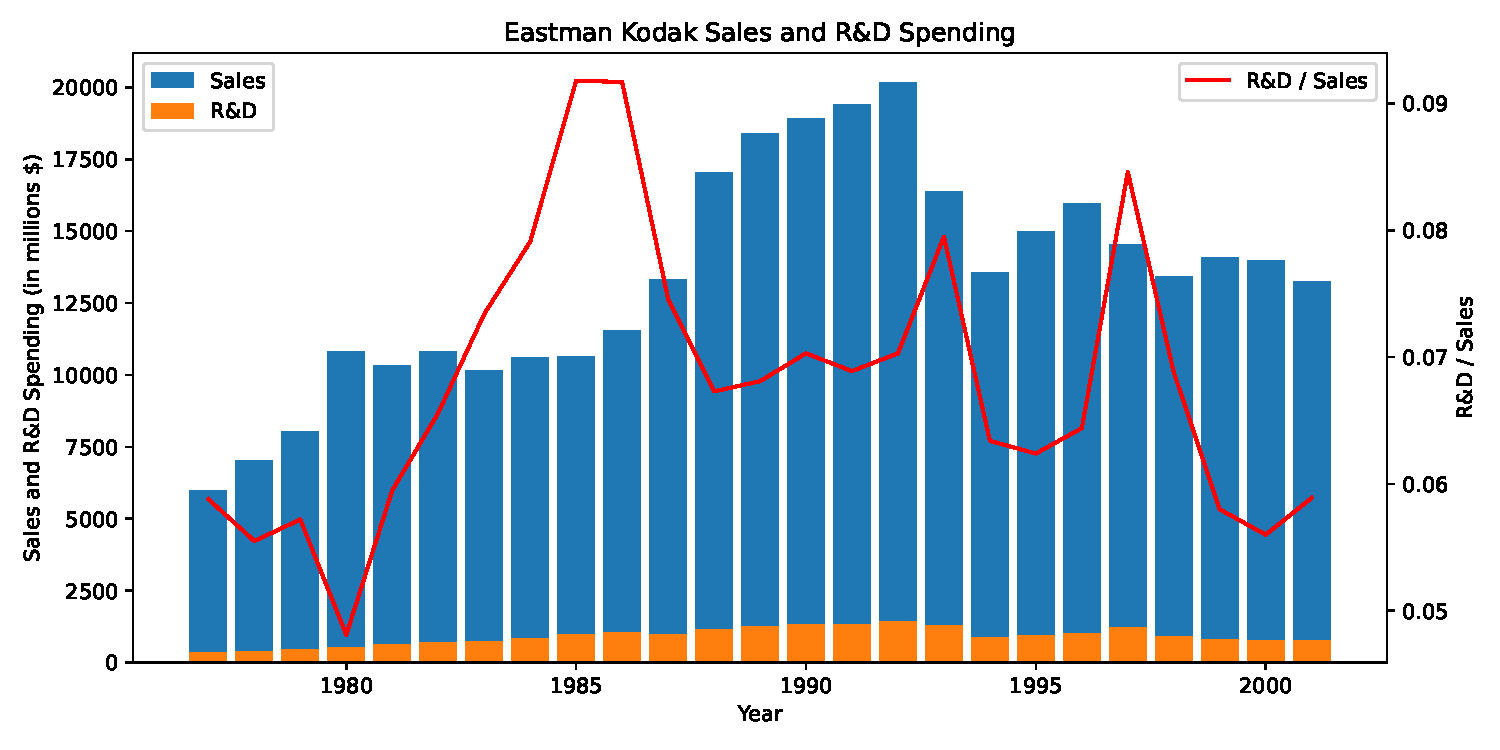
\includegraphics[width=0.8\textwidth]{Sales_and_RD.pdf}
    \caption{Overview of Kodak's sales and R\&D spending over the years}
    \label{fig:1}
\end{figure}



\section{Fisher's legacy}

As a first step, Fisher eliminated the side businesses (divests) that were considered 
to be diversification earlier in the company's life, which allowed for paying off debt 
and overall improved the company's financial situation (S\&P's rating on Kodak's debt 
raised from BBB+ to A+). In addition, he aimed for a huge reorganization of the company, 
since he believed that Kodak could \textit{“do much besides make films.”} He tried to completely 
change Kodak's “identity” from a traditional photography company to a high-tech company, 
exploiting his experience as former CEO of Motorola. This was quite idealistic and 
optimistic, since the company was already behind in digital imaging. Simultaneously 
catching up and switching market segments is one the reasons these restructurings 
failed. Another factor was that not all executives believed in Fisher's new vision 
of the company. The majority of the employees had the traditional photography mindset, 
where cameras relied on film. Fisher reformuled Kodak's vision towards high-tech 
markets, but the company (especially the senior staff and middle management) oriented 
towards producing film. As he admitted prior to his resignation, Kodak has always 
been in the picture business, and its goal should be to assist  people to do more 
with their pictures: \textit{"Electronic imaging will not cannibalize film. One of the 
mistakes we at Kodak have made is that we've tried to do it all. We do not have 
to pursue all aspects of the digital opportunity and we see our opportunity in the 
output and service side"}. Although Fisher's vision was valid, the sudden change 
and bold leadership clashed with the traditional culture of Kodak, where risks 
were usually averted. Middle managers were unable to commit to high-tech innovations, 
because this endangered short-term profit.

Moreover, Fisher entered the Chinese market, exploiting his network built 
during his time at Motorola. After only 3 years, they outperformed all competitors 
on the Chinese market (Figure 2). This endeavor not only allowed for more sales, but especially because the cheap manufacturing and acquisition of materials in these areas facilitated an efficient ecosystem. As mentioned in the case, Kodak managed to become the third firm in China in film and fourth in paper, with only 30 employees. This emphasizes the efficiency of the market cycle.

\begin{figure}[htbp]
    \centering
    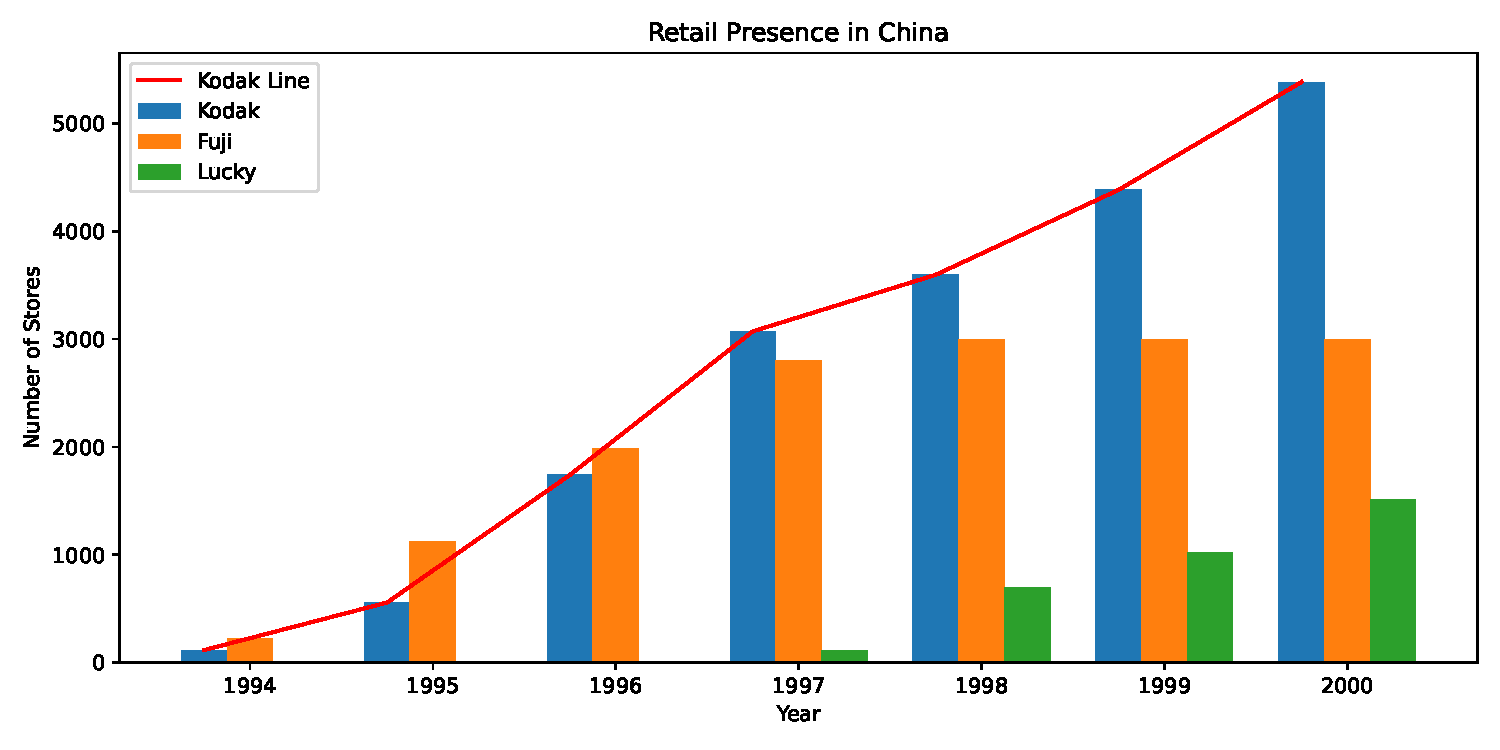
\includegraphics[width=0.8\textwidth]{retail_presence.pdf}
    \caption{Kodak's retail presence in China after appointing Fisher}
    \label{fig:2}
\end{figure}



\section{Fisher versus Carp}

Finally, the approaches of Fisher and Carp to turn the tide on Kodak's fall from a 
prominent position in the photography market are compared and the similarities and 
contradictions are looked at more deeply. Additionally, advice is given on each 
strategy in which both strategies could have improved their innovation diffusion 
of their products and services.

The similarity between Fisher's era and Carp's era is that they both shared the 
ideology that Kodak should be run as a horizontal company and as a “network of 
consumables”-based business model. However, their reasoning behind this ideology 
is different. Fisher believed that Kodak is more than just a company that is built 
on film, which resulted in a certain neglect on film altogether. As Kodak was 
working on too many things, they neglected the entrance of Fuji on the US market 
charging low prices, which resulted in radical cutbacks in Kodak of \$1.2 billion 
in costs and 19900 jobs, ending up in the resignation of Fisher (Figure 3). 
Carp believed in the synergy of both film and digital imaging and that both 
would “create a profitable bridge between the old and new worlds of photography. 
Contrarily, Fisher's approach was too digital imaging focused, which resulted 
in his resignation mentioned earlier.

Additionally, Carp shared the notion of Fisher that developments in electronics 
would result in more profits to be made for Kodak. As such, during Carp's era, 
some notable developments were made, which resulted in a number two position 
behind Sony on the market. As such one can note that Fisher paved the way for 
Carp in succeeding. While Fisher also radically revolutionized Kodak - which 
did not go smoothly - Carp did not alter the company structure to that extent. 
He did however reconstruct the digital and applied imaging fraction by merging 
it with the consumer imaging fraction, further centralizing this fraction. 
However, during Carp's era, Kodak kept making a loss of \$60 per unit camera sold. 
Carp in response kept on advertising Kodak, which is in contrast to Fisher who was 
primarily focused on building connections with different industries and relevant 
figures from his network. Carp, a veteran insider of Kodak, kept on holding 
onto one of the aspects of the old successful formula of Kodak, which states 
to 'advertise the product'.

An advice on how Fisher could improve the change of tide approach for Kodak, would be to not only radically change the company structure, but also change or add company personnel to Kodak. Fisher as an outsider was unaware of the cultural clash such a radical change could bring to Kodak, as the majority of the personnel below the top of the company was still accustomed to a razor-bladed culture which kept impeding the transition of Kodak into a true high-tech company. The mid-managers did not have the know-how of the new digital era and should have either been trained or substituted with specialists with understanding of the matter. Moreover, managers who firmly believed in the potential of the disruptive technology, would have been of great value. Concluding, Fisher did not think through the radical restructuring of Kodak properly, as the top was revolutionized but the majority of Kodak was still traditionally oriented and rather conservative. Furthermore, both Fisher and Carp made the mistake of investing their resources in R\&D but not exploiting this newly found knowledge to develop a product capable of capturing a segment of the market. As Kodak had been very tentative with this knowledge, they missed opportunities to secure a segment in the market and eventually benefitting from this fact. As such, investments in advertising and marketing done by both Fisher and Carp could have been used in the development of such opportunities. 

\begin{figure}[htbp]
    \centering
    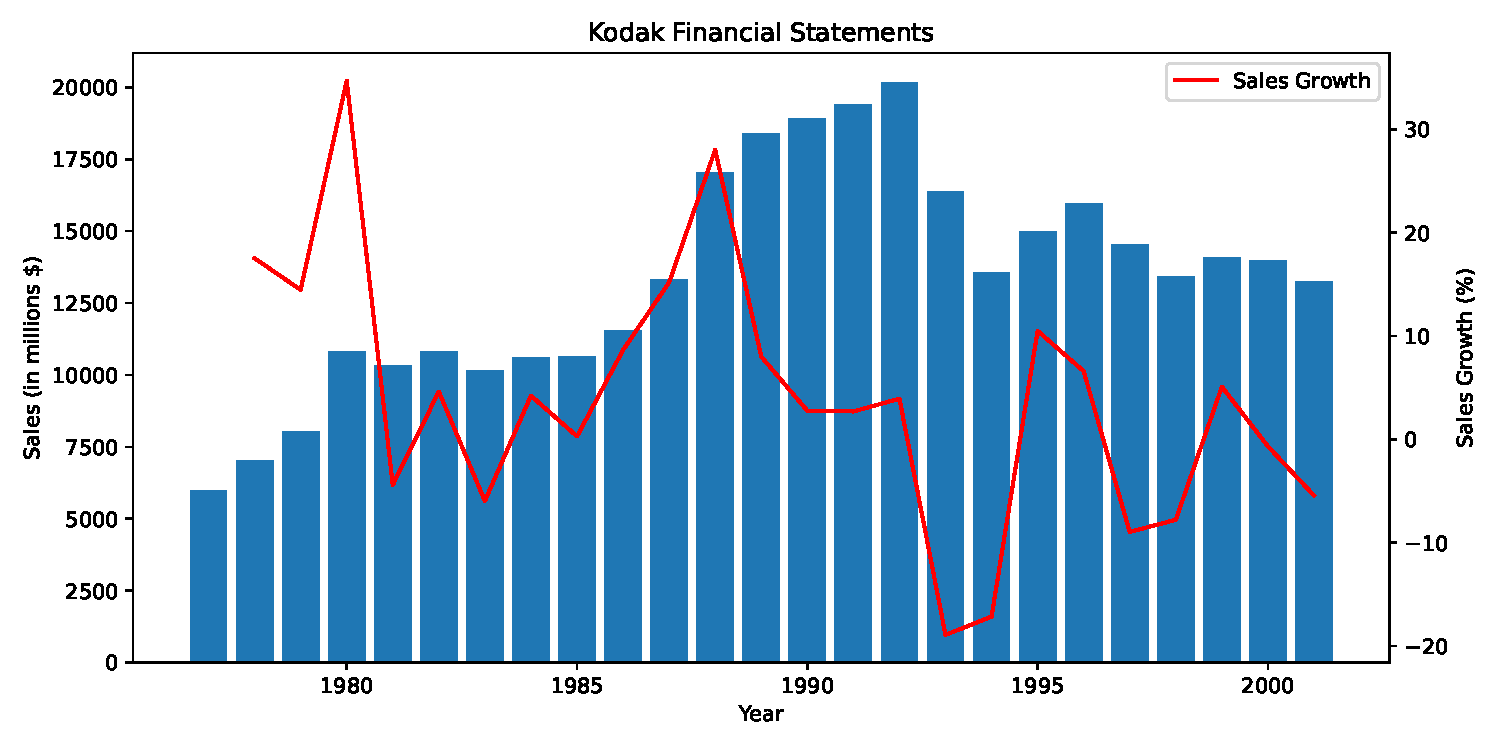
\includegraphics[width=0.8\textwidth]{Sales.pdf}
    \caption{Kodak's sales and growth rate over time}
    \label{fig:3}
\end{figure}









% % bibliography
% \bibliographystyle{ieeetr}
% \bibliography{bibl}

\end{document}